\newpage
\section{Quantum GIS}

\nocite{qgis:www}
\index{QGIS,Quantum GIS}

\begin{center}
	
\includegraphics[scale=0.1]{pictures/qgis_logo}
\end{center}

Quantum GIS je nejen prohlížečka geografických dat dostupná pro MS Windows, GNU/Linux, Unix, BSD a Mac OS X. Quantum GIS podporuje díky knihovně \index{OGR}OGR většinu vektorových formátů dat jako například ESRI Shapefile, GRASS, MapInfo či GML a díky knihovně \index{GDAL} GDAL mnoho rastrových formátů jako TIFF, ArcInfo, GRASS raster, ERDAS a další. Přes Quantum GIS můžeme také přistupovat k datům uložených v geodatabázích PostGIS a SpatiaLite či k datům dostupných přes WMS a WFS služby. Quantum GIS je šířen pod licencí GNU Public Licence. \footnote{http://qgis.org/about-qgis/features.html}

Program je napsán v jazyce C++. Poslední stabilní verze nese označení 1.7.4. Quantum GIS je lehce rozšířitelný program pomocí pluginů, které mohou být psány na jazyce Python nebo C++. Quantum GIS má poměrně dobře zdokumentované API a nutno také podotknout, že komunita kolem Quantum GISu je aktivní a podpora skrze mailinglisty je na vysoké úrovni.

Systém začal vyvíjet v roce 2002 Gary Sherman. Mělo jít o nenáročnou prohlížečku geodat pro Linux s širokou podporou datových formátů. Dlouhou dobu byl Quantum GIS brán převážně jako grafická nadstavba pro jiný desktopový GIS - GRASS GIS. Přes GRASS Plugin QGIS zpřístupňuje řadu modulů GRASS GIS. V současnosti se na vývoji nejvíce podílí skupina vývojářu kolem organizace \footnotemark{\index{Faunalia} Faunalia}\footnotetext{http://www.faunalia.co.uk/quantumgis}.

Funkcionalitu Quantum GIS rozšiřuje množství pluginů. Jako základní pluginy bych označil \footnotemark{\index{fTools} \textbf{fTools}} \footnotetext{http://www.ftools.ca/}, který umožňuje pokročilé prostorové analýzy nad vektorvovými daty, \footnotemark{\index{GDAL, GdalTools} \textbf{GdalTools}} \footnotetext{http://www.faunalia.co.uk/gdaltools} pro práci s rastrovými daty a již zmíňený \footnotemark{\index{GRASS Plugin} \textbf{GRASS Plugin}} \footnotetext{http://grass.osgeo.org/wiki/GRASS\_and\_QGIS} plugin, který zpřístupňuje funkce GRASSu uživatelům Quantum GIS. 

\subsection{Správa pluginů}
Jak už bylo zmíněno Quantum GIS umožňuje uživatelům rozšiřovat funkce programu dle jejich potřeb v podobě zásuvných modulů. Díky dobře zdokumentovanému API může uživatel pohodlně psát pluginy v jazyce C++ nebo Python. Pluginy píší jak vývojáři Quantum GISu, tak i obyčejní uživatelé. Pluginy si můžete stáhnout z oficiálních či neoficiálních repositářů. Pro instalování pluginů napsaných v jazyce Python a správu repositářů slouží nástroj \textbf{QGIS Python Plugin Installer}, dostupný přes \textit{Plugins $\rightarrow$ Fetch Python Plugins...}.

\begin{figure}
	\centering
	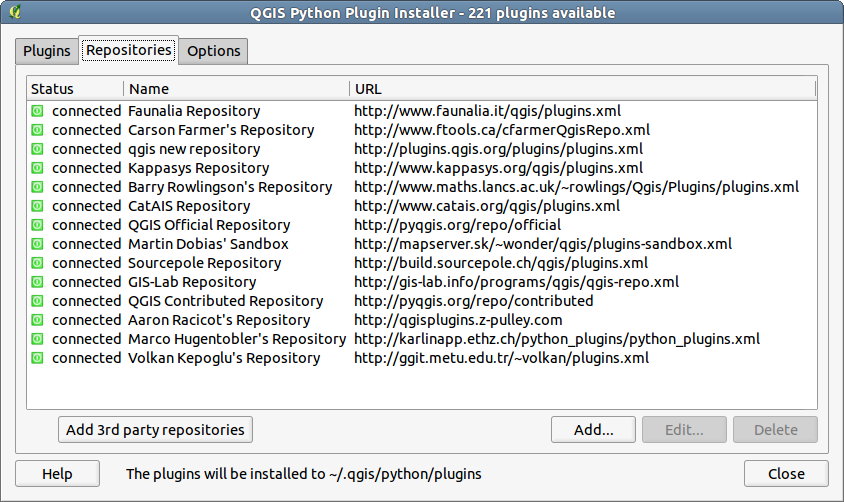
\includegraphics[scale=0.5]{pictures/qgis_plugin/python_installer}
	\caption{QGIS Python Plugin Installer - správa repozitářů}
  	\label{pythonplugininstaller}
\end{figure}


\noindent Jak je vidět z [Obr. \ref{pythonplugininstaller}], takto nainstalované pluginy se stáhnou do adresáře: 

\begin{itemize}
	\item \textit{\$HOME$\setminus$.qgis$\setminus$python$\setminus$plugins} - v případě OS GNU/Linux
	\item \textit{C:$\setminus$Documents and Settings$\setminus$USER$\setminus$.qgis$\setminus$python$\setminus$plugins} - v případě OS Windows bývá cesta podobná této
\end{itemize}

Pakliže uživatel napíše plugin v jazyce Python, doporučuji ho uložit do tohoto adresáře. Je také sice možnost uložit plugin do adresáře \textit{\$QGIS\_INSTALL\_DIR $\setminus$share$\setminus$qgis$\setminus$python$\setminus$plugins}, ale při případné opětovné kompilaci by byly změny ztraceny.

\noindent Pluginy psané v C++ se po přeložení ukládají standardně v \textit{\$QGIS\_INSTALL\_DIR $\setminus$lib$\setminus$qgis$\setminus$plugins} případně uživatel může přidat nová úložiště pomocí \textit{Settings $\rightarrow$ Options} a v záložce \textit{Generals} zadat cestu [Obr. \ref{cpprepository}].

\begin{figure}
	\centering
	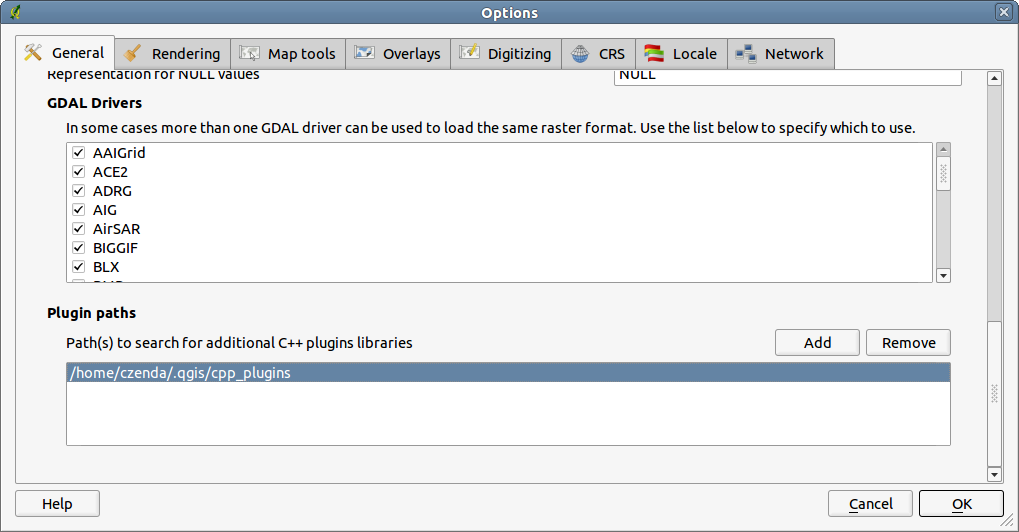
\includegraphics[scale=0.5]{pictures/qgis_plugin/options_cpp_path}
	\caption{\textit{Settings$\rightarrow$Options$\rightarrow$Generals} - přidání nové cesty k pluginům psaných na jazyce C++}
  	\label{cpprepository}
\end{figure}

Všechny nainstalované pluginy, ať psané v jazyce C++ či Python, může uživatel spravovat přes \textbf{QGIS Plugin Manager} - \textit{Plugins$\rightarrow$Manage Plugins...} [Obrázek \ref{plugin_manager}.

\begin{figure}
	\centering
	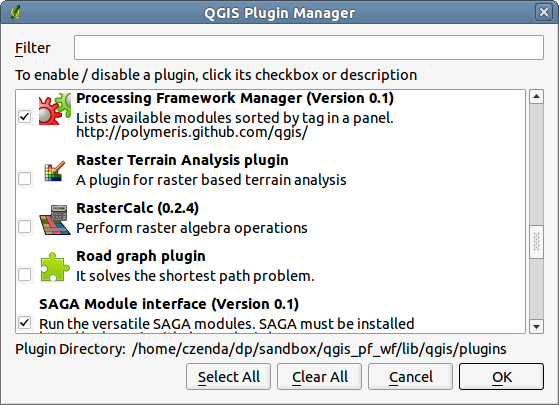
\includegraphics[scale=0.5]{pictures/qgis_plugin/plugin_manager}
	\caption{\textit{Plugins $\rightarrow$Manage Plugins...} - správa pluginů}
  	\label{plugin_manager}
\end{figure}

\subsection{Psaní vlastního pluginu}
Pluginy mohou být psány na jazyce C++ a Python. Již z charakteristiky daných jazyků vyplývá, že pro jednoduché, nenáročné či na začátku vývoje pluginy, se bude hodit spíše jazyk Python, který se nemusí kompilovat a píše se v něm rychleji než v jazyce C++. Pro rozsáhlejší projekty je lepší sáhnout po jazyce C++. Obecně jsou programy psané v kompilovaných jazycích mnohem rychlejší než programy psané v jazycích interpretovaných. 

\subsection{Python plugin}
\nocite{pyqgis:www}
\index{PyQGIS}
Při psaní pluginu v jazyce Python využíváme nástroje PyQGIS. Kromě dokumentace k Quantum GIS API také doporučuji \cite{pyqgis:www}. Dále můžeme využít nástroj Plugin Builder, což je v podstatě také plugin, který vygeneruje základní soubory, kód, který potom začneme upravovat podle tak, aby náš plugin dělal to, co chceme. \\

% dat to do prilohy
%\lstinputlisting[caption={\_\_init\_\_.py - inicializační soubor},label=plugin:init]{code/plugins/python/__init__.py}

\subsection{C++ plugin}
QGIS Processing Framework je plugin psaný v jazyce Python, proto se zde nebudu mnoho zmiňovat o pluginech psaných v jazyce C++. Více informací o tvorbě pluginů v C++ můžete najít v \footnotetext{http://download.osgeo.org/qgis/doc/manual/qgis-1.5.0\_coding-compilation\_guide\_en.pdf} \footnotemark{QGIS Coding and Compilation Guide}.
% 



